\documentclass{article}
\usepackage{geometry}
\geometry{a4paper,scale=0.9}
\usepackage[utf8]{inputenc}

\usepackage{amssymb}
\usepackage{graphicx}

\title{Rapport TP4}

\author{Rosine Rolande Simo Tegninko, 20183729\\
Yu Deng, 20151659}

\date{}

\begin{document}

\maketitle

\section*{TESTS BOITE NOIRE}\\

Dans ce test, il y a deux conditions de test requises :\\

$\cdot$ Convertir des montants uniquement entre les devises suivantes : USD, CAD, GBP, EUR, CHF, INR, AUD.

$\cdot$ Seulement accepter des montants entre [0, 10000].\\

\textbf{Pour le type de devise}\\

\textbf{$\cdot$ Classes d'équivalence}\\


Dans le code, il existe un moyen de construire des objets de type CurrencyConversion. Cela générera des objets contenant plusieurs devises, qui peuvent répondre à nos exigences de test. De plus, j'ai choisi de réutiliser le même code pour plus de commodité. La structure de base du test est la suivante. Déterminez si chaque cas de test réussit en jugeant le résultat de l'exécution de la couverture ou de l'exception levée.\\
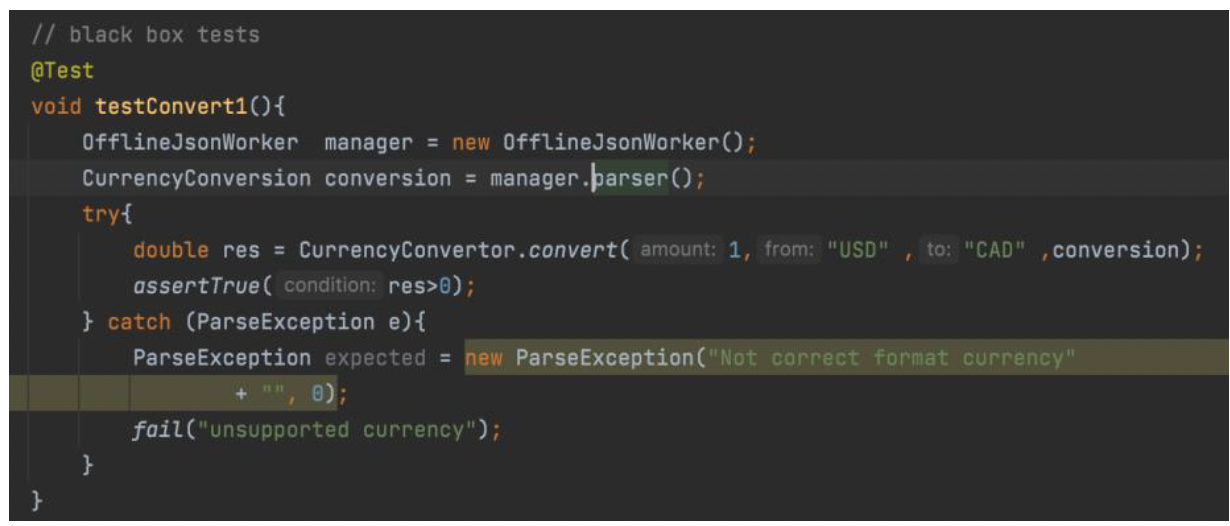
\includegraphics[scale=0.3]{G1.png}\\

Dans le cas de test 1, j'ai sélectionné USD et CAD pour la conversion. Les deux sont des types de devises qui peuvent être convertis. Cette affaire peut passer sans problème. Ensuite, j'autoriserai la conversion de sept devises pour passer le test par paires.\\
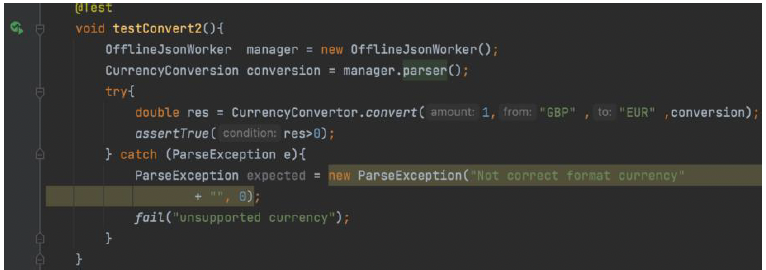
\includegraphics[scale=0.3]{G2.png}\\

Lorsque j'utilise AUD et FJD qui ne devraient pas être pris en charge pour la conversion, je trouve que l'assertion de résultat renvoie toujours le résultat normalement et j'utilise fail() pour générer des informations d'erreur, ce qui indique que convert() lui-même ne contraint pas le type de devise nous exigeons.\\
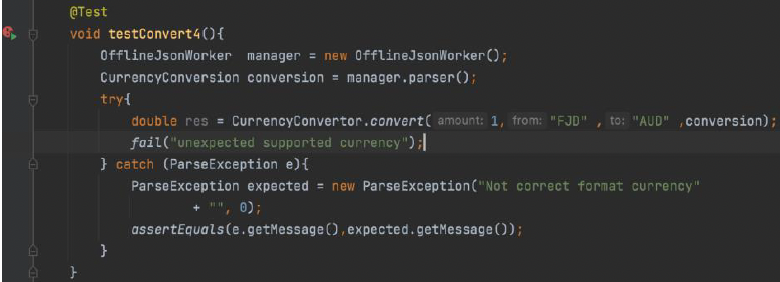
\includegraphics[scale=0.3]{G3.png}\\

\textbf{Pour plage numérique}\\

\textbf{$\cdot$ D’analyse des valeurs frontières}\\

Pour le test d'intervalle numérique, j'ai sélectionné le point final de l'intervalle, dans l'intervalle et hors de l'intervalle.\\
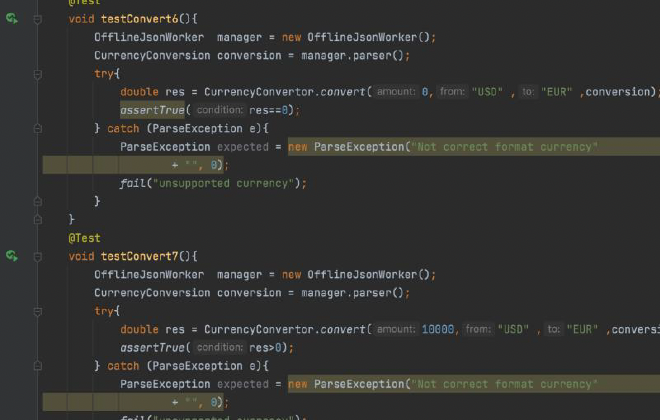
\includegraphics[scale=0.3]{G4.png} \\

Les valeurs dans l'intervalle et à la fin de l'intervalle ont passé avec succès la vérification des résultats, mais lorsque je suis allé à -1 et 10001, j'ai toujours renvoyé res normalement. En fait, ce n'est pas autorisé. Par conséquent, assertFalse échoue ici. De toute évidence, la fonction de conversion n'impose pas la limite numérique requise sur la valeur "amount".\\

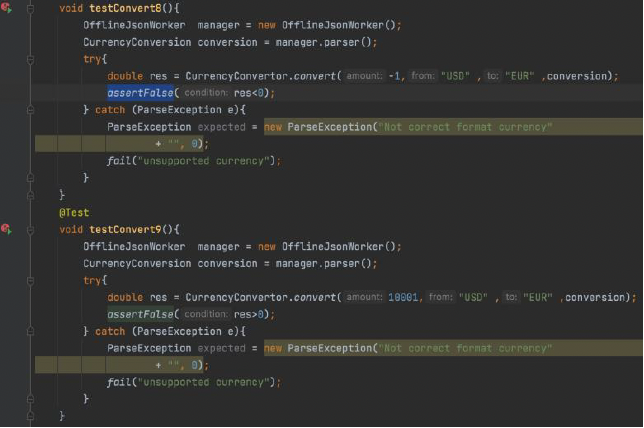
\includegraphics[scale=0.3]{G5.png}\\


\section*{TESTS BOITE BLANC}\\

Dans les tests en boîte blanche, nous devons sélectionner des cas de test significatifs en fonction de l'implémentation interne pour couvrir autant que possible différentes branches afin d'atteindre une couverture suffisante. Selon l'implémentation interne de la fonction de conversion, elle vérifie uniquement si l'objet CurrencyConversion contient le type de devise correspondant, nous allons donc nous concentrer sur l'objet CurrencyConversion pour les tests.\\

\textbf{Critère de couverture des instructions}\\
Sur la base de cette règle, nous nous concentrons sur la couverture d'exécution d'instructions spécifiques, nous devons donc proposer deux cas d'utilisation, l'un consiste à lever une exception via if, et l'autre consiste à ignorer if pour terminer l'exécution. Évidemment, ce n'est pas suffisant.\\

\textbf{Critère de couverture des arcs du graphe de flot de contrôle}\\
Pour chaque instruction conditionnelle (if, while) nous testons si la condition est vraie et si elle est fausse. ,Critère de sélection plus fort que la couverture des instructions. Parce que cette fonction est trop simple, basée sur cette règle, il n'y a pas de différence de 1.\\

\textbf{Critère de couverture des chemins indépendants du graphe de flot de contrôle}\\
Cette méthode de test accorde plus d'attention aux différents chemins complets du programme fractionné et couvre différents chemins à travers des cas d'utilisation. Il s'agit également uniquement de prendre en compte le contrôle de la direction d'écoulement des différents points de branchement, et non la situation spécifique à l'intérieur du point de branchement.\\

\textbf{Critère de couverture des conditions}\\
Cette méthode de test nécessite de considérer tous les résultats possibles dans chaque branche, non seulement pour voir si elle s'écoule vers la gauche ou vers la droite, mais aussi pour considérer quelles instances conduiront à toutes les valeurs de la condition. Même s'ils vont tous vers la gauche, plusieurs cas d'utilisation peuvent être nécessaires pour obtenir une couverture.\\

\textbf{Critère de couverture des i-chemins}\\
Cette méthode de test vise la méthode loop. Le test de fonctionnement est réalisé en contrôlant le nombre de cycles réalisés à travers différents cas d'utilisation. Ce type de contrôle de branche n'apparaît pas dans convert.\\

\textbf{Mon choix}\\
Pour résumer, nous utilisons la méthode "Critère de couverture des conditions" pour tester. De cette façon, le test peut couvrir toutes les conditions de la branche if, qui est plus adaptée, détaillée et précise que d'autres critères.
Ici, nous personnalisons certaines devises et les fausses données correspondantes pour les tests. Lorsque l'objet CurrencyConversion contient deux types de devise à convertir, le test a réussi sans problème.\\

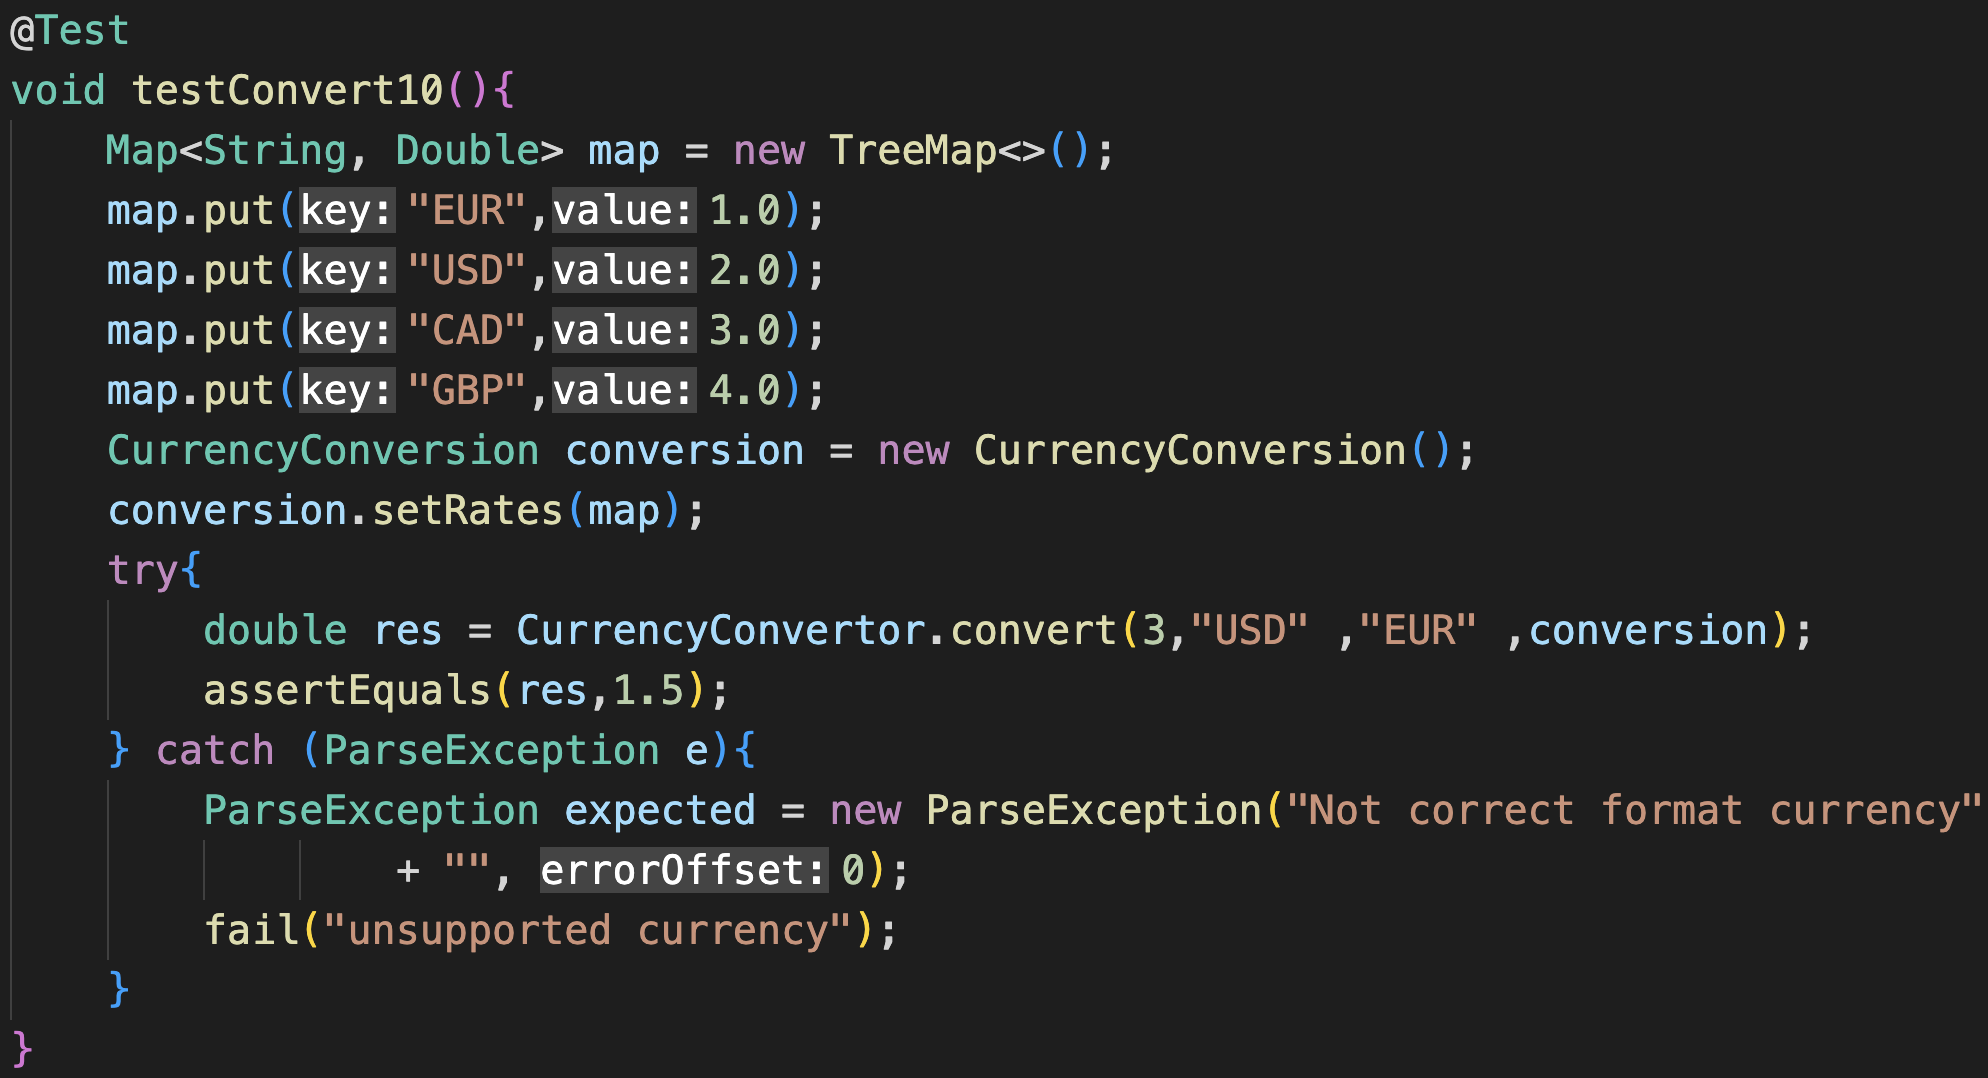
\includegraphics[scale=0.3]{G6.png}\\

Ensuite, je sélectionne les types de devises qui ne sont pas inclus dans l'objet CurrencyConversion qui sont respectivement passés dans les paramètres "from" et "to", et vous pouvez voir que l'exception attendue est levée.\\

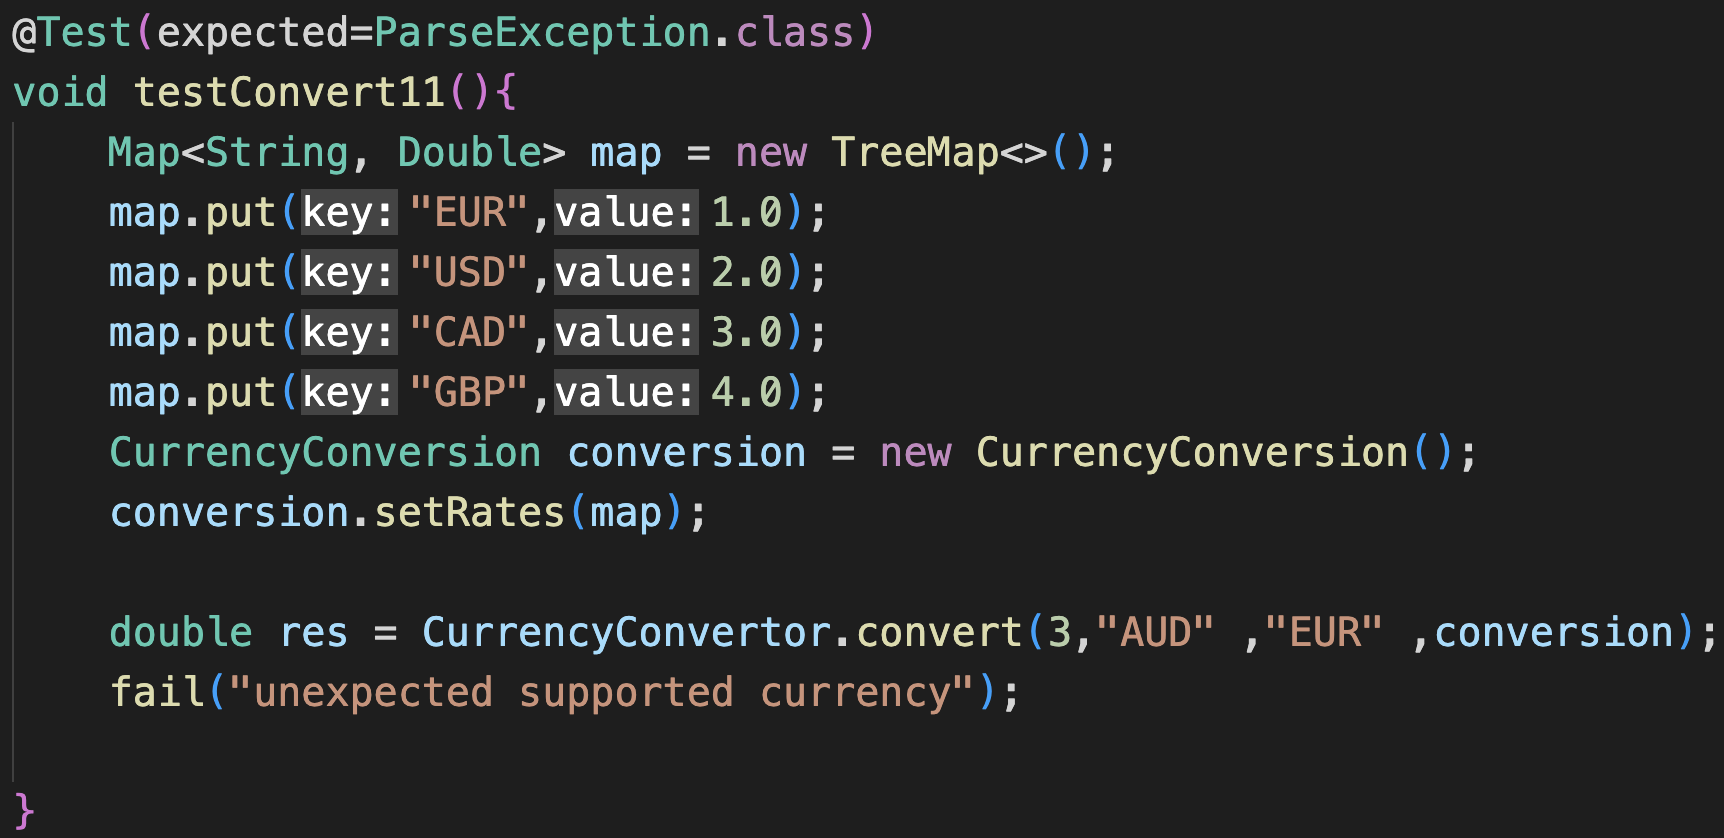
\includegraphics[scale=0.4]{G7.png}\\

En plus du paramètre CurrencyConversion lui-même, j'ai également constaté que l'opération de division s'est produite dans l'opération et qu'aucun traitement spécial n'a été effectué dans "convert". Par conséquent, j'ai défini la valeur correspondant à USD dans CurrencyConversion sur 0,0, et le test a révélé que le résultat était "Infinity".\\

\textbf{Couverture}\\

Ici, nous avons atteint une couverture de 100\% de ua. karatnyk. impl. Convertisseur de devises. convert() que nous prévoyons de tester.\\
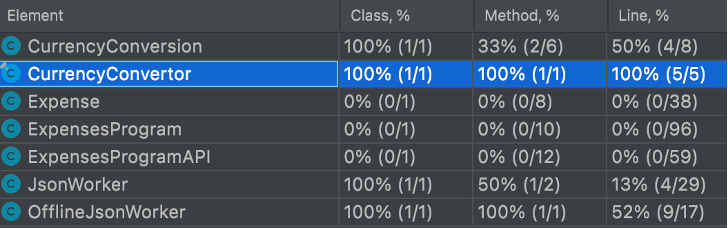
\includegraphics[scale=0.7]{G8.png}\\

\end{document}
